%This file contains the tex code of my project report for my Data Structure course.
%Author: 章凌豪 / Zhang Linghao <zlhdnc1994@gmail.com>

\documentclass[12pt]{article}
\usepackage[top=1.10in, bottom=0.75in, left=1.35in, right=1.35in]{geometry}
\linespread{1.2}
\usepackage{ctex}
\usepackage[colorlinks, citecolor=green, linkcolor=blue, menucolor=red, CJKbookmarks=true]{hyperref}
\usepackage{fancyhdr}
\usepackage{extramarks}
\usepackage{titling}
\usepackage{indentfirst}
\usepackage[linesnumbered]{algorithm2e}
\SetKw{kwNew}{\hspace{0.4em}new\hspace{0.4em}}
\SetKw{kwAnd}{\hspace{0.4em}and\hspace{0.4em}}
\SetKw{kwIn}{\hspace{0.4em}in\hspace{0.4em}}
\usepackage{graphicx}
\usepackage{array}
\usepackage{bibentry}
\usepackage{natbib}

\iffalse
\AtBeginDocument{
\begin{CJK*}{GBK}{SimSun}
\CJKindent
\sloppy\CJKspace
\CJKtilde
}
\AtEndDocument{\end{CJK*}}
\fi

\begin{document}

\pagestyle{fancy}
\lhead{\textbf{{\thetitle}}}
\rhead{\textbf{\nouppercase{\firstleftmark}}}
\cfoot{\thepage}

\title{\textbf{用DTBM进行路由表的查找和维护}}
\author{章凌豪\\13307130225}
\date{\today}
\maketitle

\tableofcontents
\clearpage

%This file contains the tex code of my project report for my Data Structure course.
%Author: 章凌豪 / Zhang Linghao <zlhdnc1994@gmail.com>

\section{问题分析}

\subsection{问题描述}

\begin{itemize}
\item 给定一个有$N(N\leq10^{7})$个表项的IPv4(或IPv6)地址路由表
\item 给出$M(M\leq10^{6})$个操作,每个操作是下列三种之一:
\begin{itemize}
\item 查找一个IP地址所对应的下一跳端口
\item 插入(若已存在则修改)一条路由表项
\item 删除一条路由表项
\end{itemize}
\end{itemize}

\subsection{要点分析}

\begin{itemize}
\item 路由转发是一个最长匹配前缀查找的过程。
\item 需要一个动态的数据结构来支持更新操作(包括增加、修改和删除),并且更新的复杂度不能太高。
\item 由于$N$较大,算法的时间复杂度最好与$N$无关。
\item 考虑到将算法拓展到IPv6地址的情形,需要考虑算法的时空复杂度是否依赖于IP地址位数$W$。
\end{itemize}

\subsection{Trie简介}

Trie,又称前缀树或字典树,是一种用于动态维护字符串的数据结构。字符串的最长匹配前缀查找就是Trie的经典应用之一。\\
\indent
在本问题中,IP地址相当于01字符串,所以解决本问题的一种最朴素的方法就是使用Binary Trie。\\
\indent
图1是将$P1$到$P9$的前缀插入Binary Trie后形成的结构。整个Binary Trie是一棵二叉树,图中的每个黑色结点都对应着一个前缀。查询操作即是从根结点按待查IP地址的对应二进制位选择左分支或右分支往下走,记录下最后一个遇到的黑色结点,其对应的前缀便是该IP地址的最长匹配前缀。更新操作则是先找到对应的结点,再将其标为黑色或标回白色。其中插入时有可能要创建新结点。\\
\indent
显然查询和更新操作都十分容易实现,且都能在$O(depth)$内完成。但简单的代价就是在最坏情况下每次操作都要走到树的最底层,可能导致性能表现不佳。而在真实世界的路由表中,/24的前缀最为常见,这意味着树的深度一般都会超过$24$。除此之外,Binary Trie中存在大量无效结点,空间使用效率极低。它在IPv4下的表现或许还不错,到了IPv6下由于地址长度增为原来的$4$倍,空间使用呈指数式上升,实用性不强。\\
\indent
朴素的Binary Trie的这些缺点催生了它的许多变种,比如我们熟知的通过将连续的白色结点压缩从而节省空间和缩短搜索路径的Path Compression Trie等。在这些变种中有一种叫做Multi-bit Trie,本报告将在第2节详述的Dynamic Tree Bitmap就是基于它发展而来的。\\
\indent
Multi-bit Trie的主要思想是通过将连续$stride$(之后简记为$S$)个结点压缩成一个结点,从而将Trie的高度从$W$压缩到$\lceil\frac{W}{S}\rceil$,达到压缩查询路径的目的。图2是图1的例子在Multi-bit Trie上形成的结构,可以看到树的高度从$5$被压缩到$2$。由于涉及到前缀扩展(prefix expansion),Multi-bit Trie的更新花费是$O(\lceil\frac{W}{S}\rceil + 2^{S})$的,空间花费为$O(\frac{2^{S}NW}{S})$。Multi-bit Trie虽然在查询上很理想,但更新花费过大,所以不适合本问题中需要面对的高度动态情形。\\

\begin{figure}[h!]
\centering
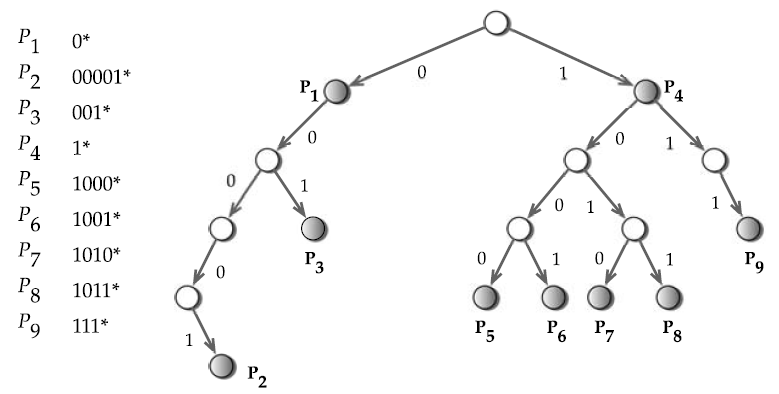
\includegraphics[scale=0.4]{trie.png}
\caption{图1}
\end{figure}

\begin{figure}[h!]
\centering
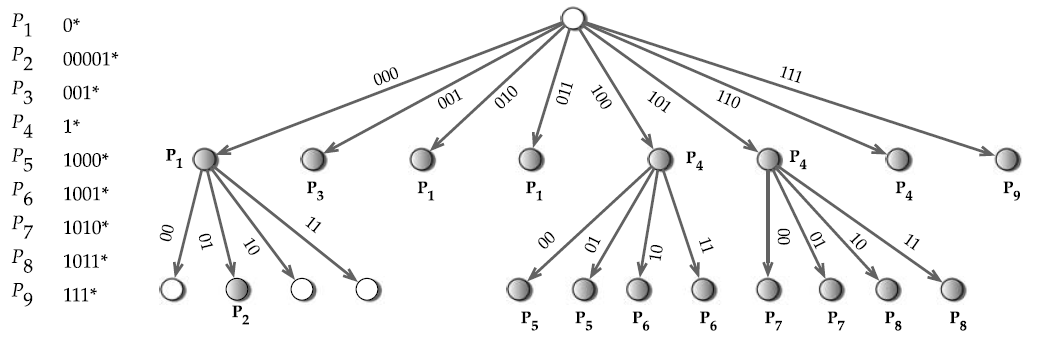
\includegraphics[scale=0.4]{mbt.png}
\caption{图2}
\end{figure}

\clearpage
%This file contains the tex code of my project report for my Data Structure course.
%Author: 章凌豪 / Zhang Linghao <zlhdnc1994@gmail.com>

\section{算法分析}

\subsection{数据结构}

本课程设计中选用的数据结构为Dynamic Tree Bitmap。这是一种基于多分支Trie的动态数据结构。\\
\indent
每个DTBM结点代表了一棵高度为$S - 1$的满二叉树。而这棵满二叉树又相当于一棵有$2^{S}-1$个结点的Binary Trie。与Binary Trie为每个结点开辟空间并用一个位标记来表示是否存在结束于当前结点的前缀不同,我们将一个DTBM结点所代表的树中的结点按层次遍历的顺序组成一个$Internal Bitmap$,它的哪一位为$1$就说明存在一条对应的前缀。\\
\indent
此外,每个DTBM结点还有一个$External Bitmap$,用于表示在多分支Trie意义下该结点的哪些位置挂着子结点。\\
\indent
图3是DTBM的一个例子:\\

\begin{figure}[h!]
\centering
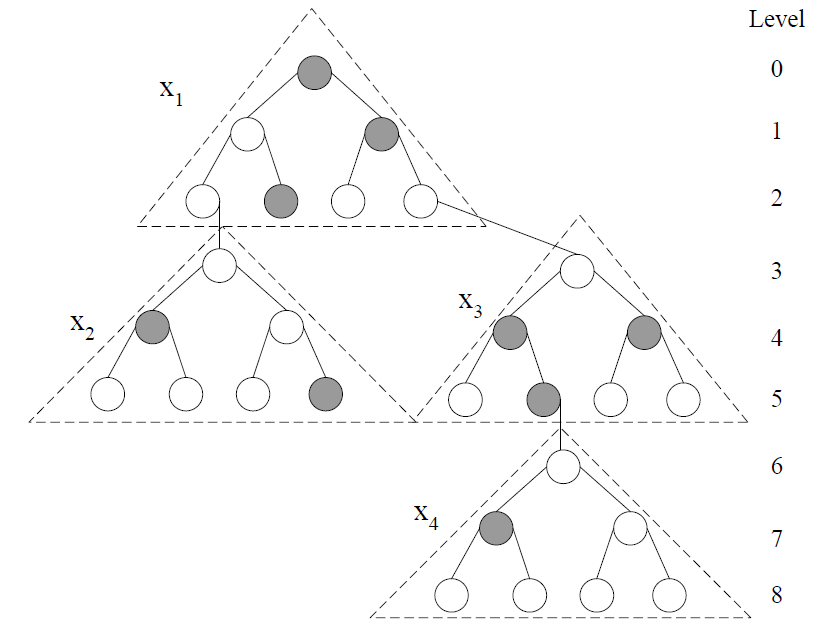
\includegraphics[scale=0.6]{dtbm_eg.png}
\caption{图3}
\end{figure}

\indent
在实际实现时,每个DTBM结点有以下域:
\begin{itemize}
\item $IBM$:用于记录$Internal Bitmap$。在DTBM的实现中,IBM是一个整型,它在二进制表示下的每一位标记了对应前缀的存在与否。
\item $EBM$:用于记录$External Bitmap$。在DTBM的实现中,$EBM$由$2^{S}$个指向子结点的指针组成。
\item $count$:用于记录该结点有多少个$EMB$指针。
\item $nextHop$:用于记录该结点中存在的前缀所对应的下一跳端口。
\end{itemize}

\indent
图4是对应图3中的DTBM的结构。\\

\begin{figure}[h!]
\centering
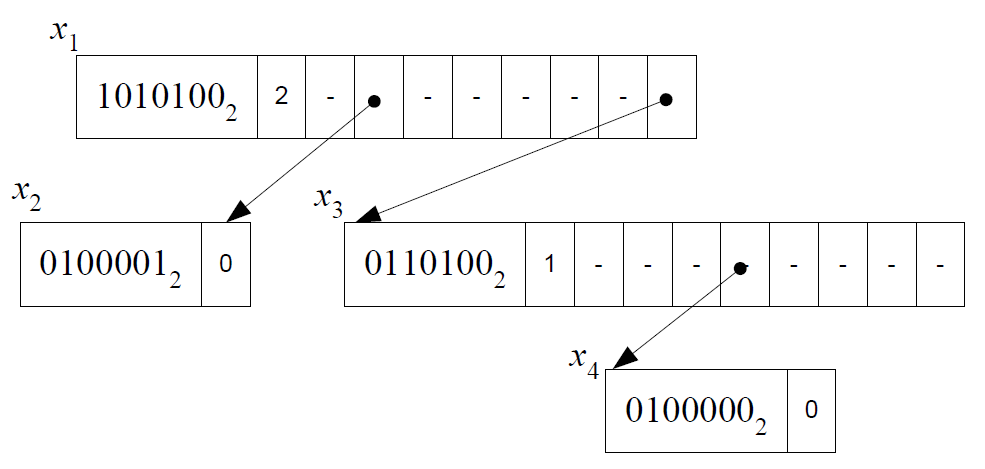
\includegraphics[scale=0.6]{dtbm_struct.png}
\caption{图4}
\end{figure}

\subsection{查找操作}

查找一个IP地址$P$时,我们从根结点出发,每次计算$P.bits(S)$在当前节点中的匹配长度$matchLength$,并检查$IBM$中对应的位是否为1。其中$P.bits(S)$表示当前$P$的前$S$位。\\
\indent
若为1,则说明当前结点中存在一个与待查找的IP地址匹配的前缀。用$bestMatch$和$hopIndex$记录下当前节点以及匹配的前缀所对应的下一跳端口在$nextHop$中的下标。\\
\indent
这一步完成后,我们通过指针$EBM[P.bits(S)]$移动到对应于$P.bits(S)$的子结点,并将$P$左移$S$位。\\
\indent
如此反复,直到走到一个空结点为止。\\
\indent
此时$bestMatch$中储存的即为最后也是最长的一个与待查的IP地址匹配的前缀所在的结点。利用$hopIndex$即可获取查询结果。\\
\indent
其中$matchLength$的求法如下:\\
\indent
对于给定的$P.bits(S)$,它所对应的结点$i$在树中的位置是$2^{H} + P.bits(H)$。其中$H$是树的高度,显然$H = S - 1$。\\
\indent
如果树中存在某一长度的与$P$匹配的前缀,那一定在$i$到根的路径上。利用完全二叉树的性质,$i$的父结点的下标可以简单地由$i/2$得到。\\
\indent
算法如下:

\begin{algorithm}
\NoCaptionOfAlgo
\caption{$Lookup(P)$}
	\Begin{
		$currentNode \leftarrow root$\;
		\Repeat{$currentNode = null$}{
			$matchLength \leftarrow currentNode.IBM.Match(P)$\;
			\If{$matchLength \geq 0$}{
				$bestMatch \leftarrow currentNode$\;
				$hopIndex \leftarrow 2^{matchLength} + P.bits(matchLength)$\;
			}
			$currentNode \leftarrow currentNode.EBM[P.bits(S)]$\;
			Shift $P$ by $S$ bits\;
		}
		\KwRet{$bestMatch.nextHop[hopIndex]$}
	}
\end{algorithm}

\begin{algorithm}
\NoCaptionOfAlgo
\caption{$Match(P)$}
	\Begin{
		$i \leftarrow 2^{H} + P.bits(H)$\;
		$length \leftarrow H$\;
		\While{$i > 0 \kwAnd IBM(i) = 0$}{
			$i \leftarrow i / 2$\;
			$length \leftarrow length - 1$\;
		}
		\KwRet{$length$}\;
	}
\end{algorithm}

\subsection{插入操作}

插入一个前缀$P$时,我们先一边左移$P$一边往下走,直到$P$的长度不足$S$或是当前节点不存在对应$P.bits(S)$的$EBM$指针为止。\\
\indent
如果是后面一种情况,我们就要创建新的结点,直到$P$的长度不足$S$为止。这时要注意设置对应的$EBM$指针并更新$EBM$指针的计数。\\
\indent
然后就可以将$P$插入到当前结点。类似地,$P.bits(P.length)$在$IBM$中对应的下标为$i = 2^{P.length} + P.bits(P.length)$。\\
\indent
算法如下:

\begin{algorithm}
\NoCaptionOfAlgo
\caption{$Insert(P)$}
	\Begin{
		\If{$root = null$}{
			$root \leftarrow \kwNew Node$\;
		}
		\While{$P.length \geq S \kwAnd currentNode.EMB[P.bits[S]] \neq null $}{
			$currentNode \leftarrow currentNode.EBM[P.bits[S]]$\;
			Shift $P$ by $S$ bits\;
		}
		\If{$P.length \geq S$}{
			$currentNode.count \leftarrow currentNode.count + 1$\;
			\Repeat{$P.length < S$}{
				$currentNode.EBM[P.bits[S]] \leftarrow \kwNew Node$\;
				$currentNode \leftarrow currentNode.EBM[P.bits[S]]$\;
				$currentNode.count \leftarrow 1$\;
				Shift $P$ by $S$ bits\;
			}
		}
		Insert $P$ into $currentNode$\;
	}
\end{algorithm}

\subsection{删除操作}

删除一个前缀$P$时,可能出现由于$P$的删除导致一条链上的结点都成为空结点而需要删除的情况。\\
\indent
所以我们在往下走时要将所有$count = 1$且$IBM = 0$的结点都记录下来,因为当这一条链的末尾被删除后,这些结点既不记录前缀,也没有了$EBM$指针,就成为了空结点。\\
\indent
注意在往下走时只要遇到一个不满足上述条件的结点,最后就不需要删除整条链。我们用$nonWeakNode$记录这个结点。\\
\indent
除此之外删除操作与插入操作大致相同,算法如下:

\begin{algorithm}
\NoCaptionOfAlgo
\caption{$Delete(P)$}
	\Begin{
		$currentNode \leftarrow root$\;
		$nonWeakNode \leftarrow null$\;
		\While{$P.length \geq S \kwAnd currentNode \neq null$}{
			\If{$currentNode.count = 1 \kwAnd currentNode.IBM = 0$}{
				Push $currentNode$ and $P.bits[S]$ into stack\;
			}
			\Else{
				Empty the stack\;
				$nonWeakNode \leftarrow currentNode$\;
			}
			$currentNode \leftarrow currentNode.EBM[P.bits[S]]$\;
			Shift $P$ by $S$ bits\;
		}
		\If{$currentNode \neq null \kwAnd P \kwIn currentNode$}{
			Delete $P$ from $currentNode$\;
			\If{$currentNode.count = 0 \kwAnd currentNode.IBM = 0$}{
				Delete empty nodes and set corresponding EBM pointers to $null$\;
			}
		}
	}
\end{algorithm}
	
\subsection{时空复杂度分析}

从理论上讲,选用步长$S$可以将树的高度压缩到$\lceil\frac{W}{S}\rceil$,从而使得各项操作最多只要访问$O(\lceil\frac{W}{S}\rceil)$个结点即可完成。在此基础上还有一些其他因素影响到不同操作的耗时:
\begin{itemize}
\item 对于查询操作来说,在每个结点内需要计算$matchLength$,每次最多要进行$H$次位比较,对耗时影响不大。
\item 对于插入和删除操作来说,由于需要申请和释放内存空间,涉及到如何管理内存的问题,将在3.3节中讨论。但由于数据规模并不大,所以简单地使用\textbf{malloc()}和\textbf{free()}来管理内存也不会成为性能的瓶颈。
\end{itemize}
总的来说,各项操作的复杂度基本相同。在实现中由于选用$S = 5$,所以树的高度被压缩到了$7$,虽然与朴素的Binary Tree相比,DTBM的各项操作在常数上会大一些,但整体性能还是十分优秀的。\\
\indent
由于DTBM动态维护结点,所以很难精确地计算空间消耗,但根据DTBM结点的结构可以知道空间复杂度大致是$O(2^{S}N')$的,其中$N'$是结点数。一般情况下$N' < N$,且根据路由前缀的密集程度不同,$N'$有可能会很小。极端情况下,对于每个前缀我们都要创建一条到树底的链,所以$N'$的上限是$\lceil\frac{W}{S}\rceil N$,在实际中这个上限是完全不可能达到的。\\
\indent
经过实际数据测试后发现,DTBM的空间消耗是完全可以接受的。\\
\indent
当将算法拓展到IPv6地址时,我们会发现除了$W$从$32$变为$128$以外,其他的一切都不需要变动。假设我们继续使用$S = 5$,树的高度就是$26$,变为原来的$4$倍左右,所以各项操作的常数会乘上一个$4$,仅此而已。\\
\indent
类似地,空间消耗也会随之增加。此时在比较坏的情况下,空间的确有可能会成为一个瓶颈,但现实情况是当前IPv6路由表项数目还非常少。当有一天IPv6路由表项数目逼近现在的IPv4路由表项数目时,新的算法自然会应运而生。\\

\clearpage

%This file contains the tex code of my project report for my Data Structure course.
%Author: 章凌豪 / Zhang Linghao <zlhdnc1994@gmail.com>

\section{实现细节}

\subsection{合理利用位运算}

DTBM是一个基于Bitmap的数据结构,所以我们可以使用一些位运算的技巧来提高程序的性能。主要有以下几点:
\begin{itemize}
\item 若要判断$IBM$的第$pos$位是否为$1$,只要看$IBM \& (1 << (pos)) = 1$是否成立即可。
\item 同样,在将前缀插入到$IBM$的第$pos$位或从$IBM$中删除第$pos$位的前缀时,简单地使用$IBM \&= \sim(1 << pos)$或$IBM \|= (1 << pos)$即可。
\item 由于算法中会频繁用到$P.bits(x)$,可以在读入数据后将$P$的二进制表示的每$S$位所对应的十进制数存入$bits[]$中,之后可以方便地由$P.bits(x) = bits[idx] >> (S - x)$来得到需要的值,其中$idx$是一个在对$P$移位时用于记录当前移到了第几个长为$S$的块的变量。
\item 对于下一跳端口,我们可以用一个\textbf{unsigned}类型来储存它。每8位可以储存一个\textbf{char},输出时,用$nxt\_hop \& (hop\_t)(unsigned char)(-1)$将除最低8位以外的位都遮盖掉,并且每输出一个\textbf{char}就将$nxt\_hop$右移8位。本问题中由于端口最多只有两个字母,所以使用\textbf{unsigned short}来储存即可。
\end{itemize}

\subsection{选择合适的步长}

步长$S$的选择是一个取舍的过程。$S$取得越大,树的高度就越小,各项操作就完成得越快,但与此同时空间占用也成倍增长。反之亦然。\\
\indent
在实现时,$S = 5$是一个不错的选择。这是因为$S = 5$对应的$IBM$位数$2^{2^{S}}=2^{32}$正好能用一个\textbf{unsigned long}存下。若令$S = 6$,虽能将树的高度再减少一层,但这就需要用\textbf{unsigned long long}来储存$IBM$,而众所周知\textbf{long long}要慢上许多。实际尝试之后也发现$S = 6$时性能与$S = 5$时相比并没有显著提升,还多占用了空间。\\
\indent
让$S = 5$还有另一个好处。在实际中/24的路由前缀是最常见的,而长为$24$的前缀正好能够落在第五层的结点,这使大部分查询都能有不错的性能表现。\\

\subsection{内存管理}

一般来讲,在实现像DTBM这样的动态数据结构时,应当使用一些内存管理的技巧。比如一次申请大块内存空间比分多次申请小块内存空间要来得快,所以我们可以在程序开始时直接申请一大块内存空间,在创建结点时即可直接使用这些分配好的内存空间。然而由于本问题中数据规模并不大,程序也并不是真正地持续运行在一台路由器上,所以在尝试以后发现并没有必要使用这些技巧。\\
\indent
现在假设我们要解决的是一个实际的工程问题,那么有这样一些技巧可以考虑使用:
\begin{itemize}
\item 维护一条可用结点链,创建结点时直接返回一个空结点供使用,删除结点时将数据清空后加到链上。
\item 如果内存足够,可以事先分配好所有结点的空间,并使用惰性操作(lazy operations),比如删除时不真正删除而是给结点打上删除标记等。
\item 通过alignment或是cache coloring之类的策略来使缓存得到充分利用,从而加快查询速度。
\end{itemize}

\clearpage
%This file contains the tex code of my project report for my Data Structure course.
%Author: 章凌豪 / Zhang Linghao <zlhdnc1994@gmail.com>

\section{性能分析}

\subsection{测试环境}

\begin{itemize}
\item \textbf{CPU:} Core i7-3615QM @ 2.30Ghz
\item \textbf{Memory:} DDR3 4GB @ 798.1Mhz
\item \textbf{System:} Windows 7 SP1
\item \textbf{Complier:} GCC 4.6.3
\item \textbf{Complier Parameter:} gcc -lm -O2
\end{itemize}

\subsection{测试结果}

\begin{table}[h]
\centering
\begin{tabular}{|l|l|l|l|l|l|}
\hline
\textbf{数据} & \textbf{总耗时} & \textbf{读入耗时} & \textbf{N} & \textbf{结点数} & \textbf{操作分布} \\ \hline
\textbf{RIB1/oper1} & 1.776s & 0.953s & 530893 & 373469 & 80\%查找/10\%插入/10\%删除 \\ \hline
\textbf{RIB1/oper2} & 1.758s & 0.966s & 530893 & 373469 & 60\%查找/20\%插入/20\%删除 \\ \hline
\textbf{RIB2/oper3} & 1.768s & 0.958s & 554528 & 151548 & 80\%查找/10\%插入/10\%删除 \\ \hline
\textbf{RIB2/oper4} & 1.563s & 0.943s & 554528 & 151548 & 40\%查找/30\%插入/30\%删除 \\ \hline
\end{tabular}
\caption{各组数据测试结果}
\end{table}

\begin{table}[h]
\centering
\begin{tabular}{|l|l|l|l|}
\hline
\textbf{数据} & \textbf{查询} & \textbf{插入} & \textbf{删除} \\ \hline
\textbf{RIB1} & 217ns & 301ns & 400ns \\ \hline
\textbf{RIB2} & 399ns & 281ns & 466ns \\ \hline
\end{tabular}
\caption{各项操作平均耗时}
\end{table}

\subsection{数据说明与分析}

\begin{itemize}
\item 表1是使用\textbf{clock()}函数计时得到的。读入耗时包括对输入进行格式处理所花的时间。
\item 表2是使用\textbf{gprof}分析得到的。插入操作包括对已有的表项进行修改的情况。
\item 由于单次操作耗时过短,各种测时和分析工具都会不可避免地积累一定的误差。所以数值上比较接近的数据之间的相对关系意义并不是太大,但还是可以看出大体情况。
\item 从大体上来讲,读入和预处理占去了一半的耗时(Windows下读入比较慢,且读入耗时与硬盘速度也有很大关系),剩下的一半时间由载入RIB和处理操作以约$1:2$的比例分别占去,这个比例也与$N$和$M$的比例相符。
\item 由表2知查询、插入、删除三项操作耗时相差不大,与2.5节中的分析较为符合。
\end{itemize}

\clearpage
\section{参考文献}

\nobibliography{ref}
\begin{enumerate}
\item\bibentry{medhi2010network}
\item\bibentry{sahni2007dynamic}
\item\bibentry{wang2009memory}
\end{enumerate}
\bibliographystyle{plainnat}

\clearpage

\end{document}
